\documentclass[10pt,xcolor={usenames,dvipsnames,table},aspectratio=169]{beamer}
\usepackage{tri_preamble}

%----------------------------------------------------------------------------------------
%	TITLE PAGE
%----------------------------------------------------------------------------------------

\title{Minimax lower bound for 1-bit Matrix Completion} 

\author{Tri Nguyen} 
\institute[OSU] 
{
    Reading group - Summer 2022 \\
Oregon State University 
% \medskip
% \textit{nguyetr9@oregonstate.edu \endgraf } 
% }
}
\date{\today} % Date, can be changed to a custom date


\makeatletter
\makeatother


\begin{document}

\frame{\titlepage}


\begin{frame}
    \frametitle{Main References}
    \begin{itemize}
        \item \fullcite{duchi2016lecture}
        \item \fullcite{scarlett2019introductory}
        \item \fullcite{Tsybakov:1315296}
        \item \fullcite{davenport20141}
    \end{itemize}
\end{frame}

\begin{frame}
    \frametitle{Recap: General Setting}
    \begin{itemize}
        \item From a distribution family $\mathcal{P} = {\blue \mathcal{N}_d = \set{N(\theta, I_d) | \theta \in \mathbb{R}^{d}}}$, God chooses a distribution $P \in \mathcal{P}$.
        \item A set of $N$ (i.i.d) samples $X_1^{N}$ are drawn from  $P$, denoted as $\bm{X}$.
        \item Task: estimating $\theta(P)$ from given samples. 
        \item Quality of estimator $\widehat{\theta}$ is measured by $\Phi(\rho(\theta, \widehat{\theta})) {\blue = \norm{\theta - \widehat{\theta}}^2}$, where:
            \begin{itemize}
                \item $\theta = \theta(P)$  is {\blue expectation} of $P = {\blue N(\theta, I_d)}$
                \item  $\widehat{\theta} = \widehat{\theta}(X_1^{n})$ is the estimator of interest. Examples: $n^{-1}(\sum^{n}_{i=1} X_i )$, $X_1$.
                \item $\Phi(t)  {\blue = t^2}$ is a non-decreasing function
                \item $\rho(\theta, \widehat{\theta}) {\blue = \norm{\theta - \widehat{\theta}}}$ is a semimetric
            \end{itemize}
        \item Question: What would be the best performance of an ideal estimator in the worse case?
    \end{itemize}
    \[
    \mathcal{M}_n(\theta(\mathcal{P}), \Phi \circ \rho) := \inf_{\widehat{\theta}} \sup_{P \in \mathcal{P}} \mathbb{E} \left[  \Phi(\rho(\theta, \widehat{\theta})) \right]
    \] 
    Finding exact $\mathcal{M}()$ is difficult, instead our attempt is to find a lower bound of it.
    % WHY, MOTIVATION?
\end{frame}


% \begin{frame}
%     \frametitle{Let's start with an example}
%     \begin{itemize}
%         \item Given a family of Gaussian $\mathcal{N}_d = \set{N(\theta, \sigma^2 I_d) | \theta \in \mathbb{R}^{d}}$.
%         \item God chooses a distribution $P \in \mathcal{N}_d$.
%         \item A set of $n$ i.i.d samples are drawn from  $P$. 
%         \item Task: estimate the mean $\theta$ from $n$ samples.
%         \item Quality of estimator is measured by $ \mathbb{E}\left[  \norm{\theta - \widehat{\theta}}^2\right]$
%     \end{itemize}
% What could be the best performance in the worse case scenario?
% \begin{itemize}
%     \item If $d=1$, we can use Cramer-Rao lower bound.
%     \item Sample mean estimator have the error of  $\dfrac{d\sigma^2}{n}$, let's see if this error can be improved.
% \end{itemize}
% \end{frame}

\begin{frame}
\frametitle{Recap: General Approach to Find Lower Bound}   
    \[
    \mathcal{M}_n(\theta(\mathcal{P}), \Phi \circ \rho) := \inf_{\widehat{\theta}} \sup_{P \in \mathcal{P}} \mathbb{E} \left[  \Phi(\rho(\theta, \widehat{\theta})) \right]
    \] 
    \begin{itemize}
        \item Translate to probability (Markov inequality)
            \[
            \inf_{\widehat{\theta}} \sup_{P \in \mathcal{P}} \mathbb{E} \left[  \Phi(\rho(\theta, \widehat{\theta})) \right]
            \geq \Phi(\delta) \inf_{\widehat{\theta}} \sup_{P \in \mathcal{P}} \mathbb{P}(\rho(\theta, \widehat{\theta}) \geq \delta)
            \] 
        \item Reduce the whole space $ \mathcal{P}$ to a finite set $\set{\theta_v| v \in \mathcal{V}}$ 
            % \[
            % \sup_{P \in \mathcal{P}}  \mathbb{P}(\rho(\theta, \widehat{\theta}) \geq \delta) \geq \dfrac{1}{\abs{\mathcal{V}}} \mathbb{P}(\rho(\theta_v, \widehat{\theta}) \geq \delta)
            % \] 
            \[
            \inf_{\widehat{\theta}} \sup_{P \in \mathcal{P}}  \mathbb{P}(\rho(\theta, \widehat{\theta}) \geq \delta) 
            \geq \inf_{\widehat{\theta}} \max_{v}\; \mathbb{P}(\rho(\theta_v, \widehat{\theta}) \geq \delta)
            \] 
        \item Reduce to a hypothesis testing error by constructing $2\delta$-\textbf{packing set}. 
            \[
            \inf_{\widehat{\theta}} \max_{v} \mathbb{P}(\rho(\theta_v, \widehat{\theta}) \geq \delta) 
            \geq \inf_{\Psi} \max_{v} \mathbb{P}(v \neq \Psi(\widetilde{X}_1^{n})),
            \] 
            where $\Psi(\widetilde{X}_1^{N}) \triangleq \argmin_{v} \rho(\theta_v, \widehat{\theta}(\widetilde{X}_1^{N}))$
        % \item Finding concrete bound based on specific problems.

    \end{itemize}
\end{frame}
\begin{frame}
    \frametitle{Recap}
    \begin{itemize}
        \item Fano's method is to switch to the average.
            \begin{align*}
\inf_{\Psi} \max_{v} \mathbb{P}(v \neq \Psi(\widetilde{X}_1^{n}))
            &\geq \inf_{\Psi} \dfrac{1}{\abs{\mathcal{V}}} \sum_{v} \mathbb{P}(v \neq \Psi(\widetilde{X}_1^{N})) \\
            &= \inf_{\Psi} \mathbb{P} (V \neq \Psi(\widetilde{X}_1^{N})), \quad \text{where $V$ is a uniform RV.}
            \end{align*} 
    \begin{lemma}
     For any discrete RVs $V, V'$ on the same alphabet  $\mathcal{V}$   ,
     \[
     \mathbb{P}(V \neq V') \geq 1- \dfrac{I(V;V') + \log 2}{\log \abs{\mathcal{V}}}
     \] 
     where $ \mathbb{P}$ is taken with respect to both $V, V'$.
    \end{lemma}
    \item There are other alternatives which do not consider RV $V$  \citep{Tsybakov:1315296}.
    \end{itemize}
\end{frame}

\begin{frame}
    \frametitle{Recap: Fano's Method - The Recipe}
    We want to lower bound the RHS of
     \[
     \mathbb{P}(V \neq V') \geq 1- \dfrac{I(V;V') + \log 2}{\log \abs{\mathcal{V}}}
     \] 
    by construct a \textbf{packing set} $\set{\theta_v| v\in \mathcal{V}}$, such that 
    \begin{columns}
        \begin{column}{0.5\textwidth}
            \begin{itemize} 
                \item (required) $\rho(\theta_v, \theta_{v'}) \geq 2\delta \quad \forall v, v' \in \mathcal{V}$
                \item (desired) $\abs{\mathcal{V}}$ is \textit{large}
                \item (desired) $I(V; V')$ is \textit{small}
                \item In the Gaussian mean estimation example, $\abs{\mathcal{V}} \geq 2^{d}$, $I(V; V') \leq O(n \delta^2)$.
            \end{itemize}
        \end{column}
        \begin{column}{0.5\textwidth}
            \begin{figure}
                \centering
                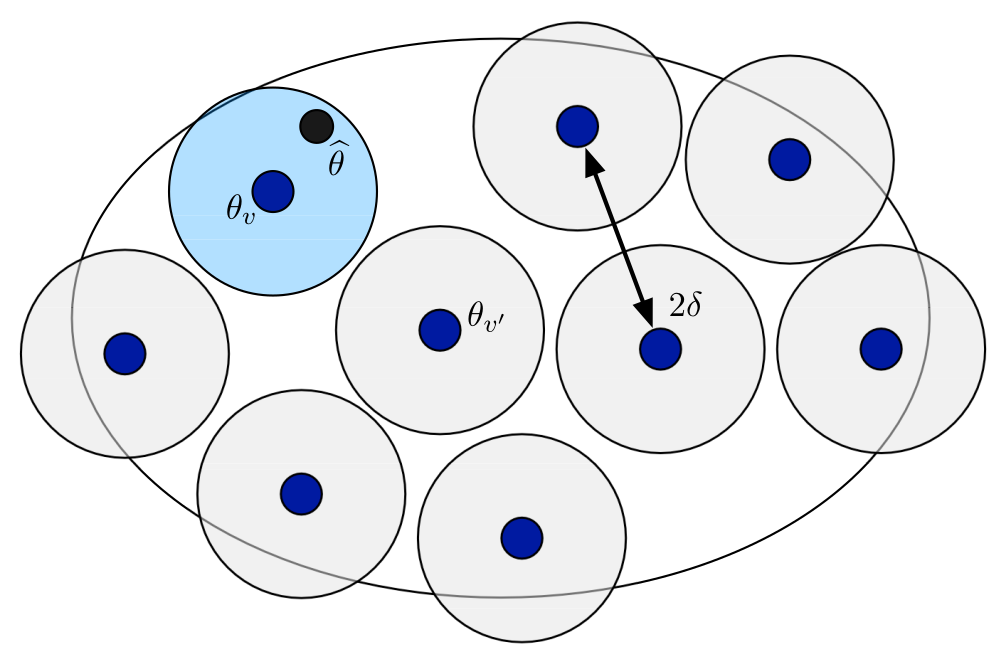
\includegraphics[width=0.5\textwidth]{figures/packing-set.png}
            \end{figure}
        \end{column}
    \end{columns}


    \textbf{Two tasks}:
    \begin{itemize}
        \item Construct packing set.
        \item Lower bound mutual information.
    \end{itemize}
\end{frame}



% \begin{frame}
%     \begin{theorem}
%         Assume that there exist $\set{P_v \in \mathcal{P}| v\in \mathcal{V}}, \abs{\mathcal{V}} \leq \infty$ such that for $v \neq v'$,  $\rho(\theta(P_v), \theta(P_{v'})) \geq 2\delta$.
%         Define
%         \begin{itemize}
%             \item $V$ to be a RV with uniform distribution over  $\mathcal{V}$, and given $V=v$ we draw $\widetilde{X}_1^{n} \sim P_v$.
%             \item For an estimator $\widehat{\theta}$, let $\Psi(X_1^{n}) := \argmin_{v \in \mathcal{V}} \rho(\theta(P_v), \widehat{\theta}(X_1^{n}))$
%         \end{itemize}
%         Then,
%         \[
%         \mathcal{M}_n(\theta(\mathcal{P}), \Phi \circ \rho) \geq \Phi(\delta) \inf_{\Psi} \mathbb{P}(\Psi(\widetilde{X}_1^{n}) \neq V)
%         \] 
%     \end{theorem}
%     \begin{lemma}[Derived from Fano inequality]
%         \[
%         \inf_{\Psi} \mathbb{P}(\Psi(\widetilde{X}_1^{n}) \neq V) \geq 1-\dfrac{I(V; \widetilde{X}_1^{n}) + \log 2}{\log \abs{\mathcal{V}}}
%         \] 
%     \end{lemma}
%     Some remarks:
%     \begin{itemize}
%         % \item This theorem bounds the minimax risk via a hypothesis testing error.
%         \item The $X_1^{n}$ in the RHS is different from the $\widetilde{X}_1^{n}$ in the LHS. $\widetilde{X}_1^{n}$ are never observed and only served for our analysis.
%         \item Choosing $\delta$ to obtain optimal lower bound. 
%             % Moreover, it is just a pseudo-data which we never actually ``touch'' it.
%         % \item In the following, $\theta_v := \theta(P_v)$, and dependence on $\widetilde{X}_1^{n}$ might be omitted.
%     \end{itemize}
% \end{frame}

% \begin{frame}
%     \frametitle{Recap: Fana's Method: The Recipe}
%     \begin{equation}
%     \label{eq:11}
%     \mathcal{M}_n(\theta(\mathcal{P}), \Phi \circ \rho) \geq \Phi(\delta) \left( 1 - \dfrac{I(V; \widetilde{X}_1^{n}) + \log 2}{\log \abs{\mathcal{V}}} \right) 
%     \end{equation}
%
%     \begin{equation}
% \label{eq:22}
%     I(V; \widetilde{\mathcal{X}}_1^{n}) \leq \dfrac{1}{\abs{\mathcal{V}}^2} \sum_{v, v' \in \mathcal{V}} D_{\rm kl}(P_v || D_{v'}) 
%     \end{equation}
%     Construct a \textit{packing set} $\set{\theta_v| v\in \mathcal{V}}$, such that 
%     \begin{columns}
%         \begin{column}{0.5\textwidth}
%             \begin{itemize} 
%                 \item (required) $\rho(\theta_v, \theta_{v'}) \geq 2\delta \quad \forall v, v' \in \mathcal{V}$
%                 \item (desired) $\abs{\mathcal{V}}$ is \textbf{large}
%                 \item (desired) $D_{\rm kl} (P_v || P_{v'})$ is \textbf{small}
%             \end{itemize}
%         \end{column}
%         \begin{column}{0.5\textwidth}
%             \begin{figure}
%                 \centering
%                 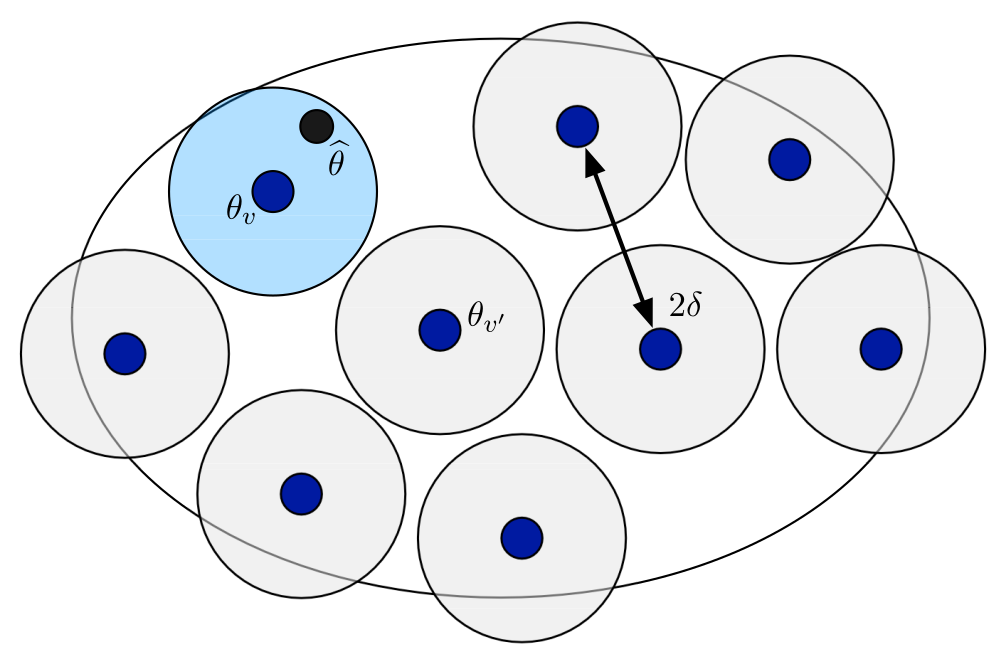
\includegraphics[width=0.6\textwidth]{figures/packing-set.png}
%             \end{figure}
%         \end{column}
%     \end{columns}
%     In Gaussian mean estimation example, $\abs{\mathcal{V}} \geq 2^{d}$, $I(V; \widetilde{X}_1^{n}) \leq O(n \delta^2)$.
% \end{frame}


\begin{frame}
    \frametitle{Minimax Bound in 1-bit Matrix Completion Problem}
\begin{itemize}
    \item Given matrix $\bm{M} \in K \triangleq \set{\bm{M}  \in  \mathbb{R}^{d_1 \times d_2} \mid \norm{\bm{M}}_{*} \leq \alpha \sqrt{r d_1 d_2}, \norm{\bm{M}}_{\infty} \leq \alpha }$.
    \item A RV $\Omega \subset [d_1] \times [d_2]$ with $ \mathbb{E}[\abs{\Omega}] = n$
    \item A differential function $f: \mathbb{R} \rightarrow [1,0]$ (cdf)
    \item Matrix $\bm{Y}$ such that
        \[
            Y_{ij} = 
            \begin{cases}
                +1 \quad & \text{with probability } f(M_{ij}) \\
                -1 \quad & \text{with probability } 1-f(M_{ij})
            \end{cases}
        \] 
    \item Task: Estimate $\bm{M}$ given $\bm{Y}, \Omega$ 
    \item Quality measurement: $\Phi(\rho(\bm{M}, \widehat{\bm{M}})) = \dfrac{1}{d_1 d_2} \norm{\bm{M} - \widehat{\bm{M}}}_{\rm F}^2$.
\end{itemize}

\begin{theorem}[\cite{davenport20141}]
        Given a fixed algorithm, there exists $\bm{M} \in K$ such that with probability at least $0.75$ {\blue (over RV $\bm{Y}$)},
        \[
        \dfrac{1}{d_1 d_2} \norm{\bm{M} - \widehat{\bm{M}}}_{\rm F}^2 
        \geq  \min \left( C_1, C_2 \alpha \sqrt{\beta_{0.75 \alpha}} \sqrt{\dfrac{r \max(d_1, d_2)}{n}}\right) = O \left(\dfrac{1}{\sqrt{n}}\right)
        \] 
\end{theorem}
Prove by construction!
\end{frame}

\begin{frame}
\frametitle{Sketch of Proof: Step 1}   
\begin{itemize}
    \item Construct a set of matrices $\mathcal{X} = \set{\bm{X}_v}$ indexed by $v \in \mathcal{V}$ such that
        \begin{itemize}
            \item $\mathcal{X} \subseteq K$
            \item $\norm{\bm{X}_v - \bm{X}_{v'}}_{\rm F}^2 \geq \epsilon^2, \quad \forall v, v' \in \mathcal{V}$ for some $\epsilon>0$.
            % \item $\abs{\mathcal{V}} = \abs{\set{\theta_v \mid v \in \mathcal{V}}}$ should be exponentially large 
            % \item $D_{kl}(P(\cdot; \theta_v) \; ||\; P(\cdot; \theta_{v'}))$ should be small
        \end{itemize}
    \item Uniformly choose a $V \in \mathcal{V}$, constructing $P(\cdot; \bm{X}_V)$, draw set $X_1^{N}$ of $N$ samples from that  $P(\cdot; \bm{X}_V)$.
    \item Let $\psi$ be the algorithm in the theorem: it uses data $\bm{Y}, \Omega$ and outputs $\widehat{\bm{M}}$.
    \item Let $\Psi$ define as  $\widehat{V} = \Psi((\bm{Y}, \Omega)) = \argmin_{v \in \mathcal{V}} \rho(\widehat{\bm{M}}, \bm{X}_v)$.
        % Fano's inequality provide such lower bound. Then if the lower is large enough, we'll get a good minimax bound.
\end{itemize}
        By construction, 
        \[
        \mathbb{P}(V \neq \widehat{V}) = \mathbb{P} \left(\norm{\bm{X}_{V} - \bm{X}_{\widehat{V}}}_{\rm F}^2 \geq \epsilon^2 \right)
        \] 
        Hence, the remaining part is to find a bound on the best possible prediction accuracy? i.e,
        \[
        \inf_{\Psi} \mathbb{P}(V \neq \widehat{V})  \geq \; q(\epsilon)
        \] 
        where $\mathbb{P}$ is respect to RVs ${\blue V, \bm{Y}_{\Omega}}$.

        Then we can claim that there exists $\bm{M}$, with probability at least $q(\epsilon)$,
        \[
        \norm{\bm{M} - \widehat{\bm{M}}}_{\rm F}^2 \geq \epsilon^2
        \] 
\end{frame}
\begin{frame}
\frametitle{Sketch of Proof:  Step 2}   
\begin{itemize}
    \item Find the lower bound of $\inf_{\Psi} \mathbb{P}(V \neq \widehat{V})$
        \begin{itemize}
            \item Fano's inequality: For any discrete RVs $V, V'$ on the same alphabet $\mathcal{V}$,
        \[
        P(V \neq \widehat{V}) \geq 1-\dfrac{I(V; \widehat{V}) + \log 2}{\log{\mathcal{V}}}
        \] 
    \item $I(V; \widehat{V}) \leq I(V; \bm{Y}_{\Omega})$ since we have a Markov chain $V \rightarrow \bm{Y}_{\Omega} \rightarrow \widehat{V}$
    \item Bound the $I(V; \bm{Y}_{\Omega})$  \citep{scarlett2019introductory}
        \begin{itemize}
            \item Tensorization if all data points are i.i.d
            \item Otherwise,
                \[
                I(V; \bm{Y}_{\Omega}) \leq \max_{v, v'} \; D_{\rm kl} (P(\cdot|v) \; || \; P(\cdot| v'))
                \] 
        \end{itemize}
        \item Upper bound that KL, which is application-dependent. Also, the $\epsilon$ should appear in this step.

        \end{itemize}
        \item Integrating everything together, choosing $\epsilon$ to have a tight/meaningful bound.
\end{itemize}
\end{frame}

\begin{frame}
    \frametitle{Step 1: Construct an Attentive Packing set}
    \begin{lemma}
        Let $\gamma \leq 1$ be such that $r/\gamma^2 \in \mathbb{N}$, and suppose that $r/\gamma^2 \leq d_1$. There is a set $\mathcal{X} \subset K$ with  
        \[
        \abs{\mathcal{X}} \geq \exp \left( \dfrac{rd_2}{16 \gamma^2} \right)
        \] 
        with the following properties:
        \begin{itemize}
            \item For all $\bm{X} \in \mathcal{X}$, each entry has $\abs{X_{ij}} = \alpha \gamma$.
            \item For all $\bm{X} \neq \bm{X}' \in \mathcal{X}$,
                \[
                \norm{\bm{X} - \bm{X}'}_{\rm F}^2 > 0.5 \alpha^2 \gamma^2 d_1 d_2
                \] 
        \end{itemize}
    \end{lemma}
\end{frame}
\begin{frame}
    \frametitle{Proof of the Existence of Packing Set}
    {\blue It is an interesting probabilistic argument.}
    
    Consider the following distribution over random matrix $\bm{X}$ with size of $d_1 \times d_2$:
     \begin{itemize}
        \item Let $d_1' \triangleq r/\gamma^2 (\leq d_1)$. 
        \item Matrix $\bm{X}$ contains multiple blocks of size $d_1' \times d_2$.
        \item For the first block, all entries are i.i.d Bernoulli RVs, i.e.,  $X_{ij} \sim \text{Bernoulli}(0.5), X_{ij} \in \set{\pm \alpha \gamma}, \forall (i,j) \in [d_1'] \times [d_2]$.
        \item For other blocks are just copies of the first block (as much as possible).
    \end{itemize}
    We will draw from this distribution to construct set $\mathcal{X}$ of $\left\lceil \exp \left( \dfrac{rd_2}{16 \gamma^2} \right)\right\rceil $ elements.


    Then $\mathcal{X} \subset K \triangleq \set{\bm{M}  \in  \mathbb{R}^{d_1 \times d_2} \mid \norm{\bm{M}}_{*} \leq \alpha \sqrt{r d_1 d_2}, \norm{\bm{M}}_{\infty} \leq \alpha }$ since
    \begin{itemize}
        \item $\norm{\bm{X}}_{\infty} = \alpha \gamma \leq \alpha$
        \item $\norm{\bm{X}}_{*} \leq \sqrt{\text{rank}}(\bm{X}) \norm{\bm{X}}_{\rm F} \leq \sqrt{d_1'} \norm{\bm{X}}_{\rm F} = \sqrt{r/\gamma^2} \sqrt{d_1d_2} \alpha \gamma = \alpha \sqrt{r d_1d_2 }$ 
    \end{itemize}

\end{frame}

\begin{frame}
    For 2 RVs $\bm{X}, \bm{Y}$ followed the above distribution,
    \begin{align*}
    \norm{\bm{X} - \bm{Y}}_{\rm F}^2 
    &= \sum_{i,j} (X_{ij} - Y_{ij})^2 \\
    &\geq \left \lfloor \dfrac{d_1}{d_1'}\right \rfloor \sum_{{i \in [d_1'], j\in [d_2]}} (X_{ij} - Y_{ij})^2  \\
    &= 4 \alpha^2 \gamma^2 \left \lfloor \dfrac{d_1}{d_1'}\right \rfloor \sum_{i \in [d_1'], j\in [d_2]} \delta_{ij} , \qquad  \delta_{ij} \sim_{\text{i.i.d}} \text{Bern}(0.5), \delta_{ij} \in \set{0, 1}
    \end{align*}
   Next, with union bound and Hoeffding's inequality, we obtain,
   \begin{align*}
   P \left( \min_{\bm{X} \neq \bm{Y}} \sum_{i \in [d_1'], j\in [d_2]} \delta_{ij} \leq 0.25 d_1' d_2\right) 
   &\leq \sum_{\bm{X} \neq \bm{Y}}  P \left( \min_{\bm{X} \neq \bm{Y}} \sum_{i \in [d_1'], j\in [d_2]} \delta_{ij} \leq 0.25 d_1' d_2\right)  \\
   &\leq {\abs{\mathcal{X}} \choose 2} \exp \left( -d_1' d_2/8 \right) {\blue < 1}
   \end{align*}
   That means that there is a non-zero probability that we obtain the set $\mathcal{X}$  such that
   \[
   \norm{\bm{X} - \bm{Y}}_{\rm F}^2 \geq \alpha^2 \gamma^2\left \lfloor \dfrac{d_1}{d_1'}\right \rfloor d_1' d_2 \geq 0.5 \alpha^2 \gamma^2 d_1 d_2
   \] 

\end{frame}

\begin{frame}
    \frametitle{Step 2: Apply Fano's Inequality}
    Let $\mathcal{X}'_{\alpha/2, \gamma}$ be the set constructed in the previous Lemma. Construct $\mathcal{X}$ as
    \[
    \mathcal{X} \triangleq \set{\bm{X}' + \alpha \left( 1 - \dfrac{\gamma}{2} \right) \bm{1} \mid \bm{X}' \in \mathcal{X}'_{\alpha/2, \gamma}},
    \] where  $\gamma$ is chosen as 
    \[
    4\sqrt{2}\epsilon/\alpha \leq \gamma \leq 8\epsilon/\alpha,
    \] 
    and $\epsilon$ is chosen such that
    \[
    \norm{\bm{X} - \bm{X}'}_{\rm F}^2 \leq 4d_1d_2\epsilon^2
    \] 
    By construction, $\mathcal{X} \subset K$ (not obvious but easy to show), and $\abs{\mathcal{X}} = \abs{\mathcal{X}'_{\alpha/2, \gamma}}$.


    % The data generating process is:
    % \begin{itemize}
    %     \item Obtain $\Omega$ where $(i,j) \in \Omega$.
    %     \item Let $\mathcal{V}$ as index set for $\mathcal{X}$.
    %     \item Draw a $V \sim \mathcal{U}$ over $\mathcal{V}$, obtain $\bm{M} = \bm{X}_{V}$.
    %     \item Draw $\bm{Y}_{\Omega}$ where $Y_{ij} $ followed $f(M_{ij})\quad \forall (i,j) \in \Omega$.
    %     \item Predict $\widehat{V}$ using $\bm{Y}_{\Omega}$.
    % \end{itemize}
    % We have a \textit{Markov chain}: $V \rightarrow \bm{M} \rightarrow \bm{Y}_{\Omega} \rightarrow \widehat{V}$, or $V \rightarrow \bm{Y}_{\Omega} \rightarrow \widehat{V}$. 
    % Fano inequality says
    % \begin{align*}
    % \inf_{\Psi} \mathbb{P} (\Psi (\bm{Y}_{\Omega}) \neq V) 
    % &\geq  1- \dfrac{I(V; \widehat{V}) + \log 2}{\log \abs{\mathcal{X}}} 
    % \end{align*}
    
\end{frame}

\begin{frame}
    \frametitle{Fano's Inequality}
    Now we show that if we choose $\bm{M} \in \mathcal{X}$ uniformly
    \[
     P(V \neq \widehat{V}) \geq 1-\dfrac{\max_{v, v'} \; D_{\rm kl} (P(\cdot|v) \; || \; P(\cdot| v'))
 + \log 2}{\log{\abs{\mathcal{V}}}}
    \] 
    By property of KL divergence of product distributions,
    \begin{align*}
        \max_{v, v' \in \mathcal{V}} D_{\rm kl} (\bm{Y}_{\Omega} |v \; || \; \bm{Y}_{\Omega}|v') 
        = \max_{v, v' \in \mathcal{V}} \sum_{(i,j) \in \Omega} D_{\rm kl} (Y_{ij}|v \; || \; Y_{ij}|v') 
    \end{align*}
    \begin{itemize}
        \item All summands are $D_{\rm KL}$ between 2 Bernoulli RVs
        \item They are either $0, D_{\rm kl} (\alpha || \alpha'), D_{\rm kl}(\alpha' || \alpha)$ (because of our construction of the packing set).
    \end{itemize}

    \begin{lemma}
        For $x,y \in (0,1), X \sim \text{Bern}(x), Y \sim \text{Bern}(y)$. Then
        \[
        D_{\rm kl} (x || y) \leq \dfrac{(x-y)^2}{y (1-y)}
        \] 
    \end{lemma}
\end{frame}

\begin{frame}
    Using the above Lemma,
    \begin{align*}
    D_{\rm kl}(Y_{ij}|v \; || \; Y_{ij}| v') 
    &\leq \dfrac{(f(\alpha) - f(\alpha'))^2}{f(\alpha')(1- f(\alpha'))}  \\
    &\leq \dfrac{(f'(\xi))^2(\alpha - \alpha')^2}{f(\alpha')(1- f(\alpha'))} \quad \text{for some } \xi \in [\alpha', \alpha] \quad (\text{intermediate value theorem})\\
    &\leq \dfrac{(\gamma \alpha)^2}{\beta_{\alpha'}} \quad (\text{since } \alpha' = (1-\gamma)\alpha)\\
    &\leq \dfrac{64 \epsilon^2}{\beta_{\alpha'}} \quad \text{(by assumption)}
    \end{align*} 
    \[
    \Rightarrow I(V; \widehat{V}) \leq \dfrac{64 n\epsilon^2}{\beta_{\alpha'}}
    \] 
    Hence,
    \begin{align*}
    \inf_{\Psi} \mathbb{P} (\Psi (\bm{Y}_{\Omega}) \neq V) 
    &\geq  1- \dfrac{I(V; \widehat{V}) + \log 2}{\log \abs{\mathcal{X}}}  \\
    &\geq 1- 1024 \epsilon^2 \left( \dfrac{64 n \epsilon^2/\beta_{\alpha'}+1}{\alpha^2 r d_2} \right)
    \end{align*}
\end{frame}

\begin{frame}
    \begin{align*}
    \inf_{\Psi} \mathbb{P} (\Psi (\bm{Y}_{\Omega}) \neq V) 
    \geq 1- 1024 \epsilon^2 \left( \dfrac{64 n \epsilon^2/\beta_{\alpha'}+1}{\alpha^2 r d_2} \right)
    \end{align*}
    Recall that 
    \[
    \norm{\bm{M} - \widehat{\bm{M}}}_{\rm F}^2 \geq 4 d_1 d_2 \epsilon ^2
    \] 
    Lastly, choose $\epsilon$ so that we get a meaningful bound. Choose
    \[
    \epsilon^2 = \ldots 
    \] 
    then they can conclude that
    \[
    \norm{\bm{M} - \widehat{\bm{M}}}_{\rm F}^2 \geq O(1/\sqrt{n})
    \] 
    with probability at least $0.75$.

\end{frame}

\begin{frame}
    \frametitle{Some Comments}
    \begin{itemize}
        \item The proof does not take into account RV $\Omega$
        \item Proof of existence of packing set using probabilistic is a nice approach
        \item Data samples does not need to be  independent
        \item Fano's inequality is a key step in the general minimax bound derivation
    \end{itemize}
\end{frame}

\end{document}
